
This section presents the theoretical foundations and detailed mechanics necessary to understand
the methods used in Section \ref{experiments}.

\subsection{Bayesian Neural Networks}
\label{methodology:bnns}
Bayesian inference allows updating prior beliefs using previously unseen data via Bayes' theorem:

\begin{equation}
P(\theta \mid \mathcal{D}) = \frac{P(\mathcal{D} \mid \theta) P(\theta)}{P(\mathcal{D})} 
\quad \text{where} \quad 
P(\mathcal{D}) = \int P(\mathcal{D} \mid \theta') P(\theta')  d\theta'
\label{eq:bayes}
\end{equation}

Here, $P(\theta)$ is the prior distribution over parameters, $P(\mathcal{D} \mid \theta)$ is the
likelihood (encoding aleatoric uncertainty), and $P(\theta \mid \mathcal{D})$ is the posterior
(capturing epistemic uncertainty) \citep{Jospin2022bnns}.
This formalism enables quantification of both uncertainty types.

\vspace{0.15cm}
Before introducing Bayesian neural networks, we briefly recall the fundamentals of standard neural
networks. Artificial neural networks (NNs) are inspired by biological brains, they consist of layered
interconnected neurons. Each neuron computes a weighted sum of inputs $x_i$ plus a bias $b$
and applies a nonlinear activation function $g(\cdot)$:

\[
z = \sum_{i} w_i x_i + b, \quad \text{output} = g(z)
\]

In a deep neural network, neurons are organized in multiple layers. During training, the network adjusts
its parameters (weights $\mathbf{W}$ and biases $\mathbf{b}$) via backpropagation and gradient
descent to minimize a loss function on training data \citep{Haykin2009, López2022anns&dl}.
These learned parameters are treated as fixed point estimates at test time, and the network produces a
single prediction without expressing uncertainty. So while NNs are powerful in pattern recognition,
they lack a mechanism to quantify confidence in their predictions.

\vspace{0.15cm}
Bayesian Neural Networks (BNNs) address this limitation by treating weights $\mathbf{W}$ as random 
variables with specified prior distributions. Given training data $\mathcal{D} = \{(x_i, y_i)\}$,
Bayes' theorem yields the posterior distribution:
% Bayesian Neural Networks (BNNs) are stochastic neural networks trained using Bayesian inference \citep[see, e.g.,][]{Jospin2022bnns}.

\begin{equation}
p(\mathbf{W} \mid \mathcal{D}) = \frac{p(\mathcal{D} \mid \mathbf{W})  p(\mathbf{W})}{p(\mathcal{D})}
\label{eq:posterior}
\end{equation}

Predictions incorporate uncertainty through marginalization over the posterior:

\begin{equation}
p(y^* \mid x^*, \mathcal{D}) = \int p(y^* \mid x^*, \mathbf{W})  p(\mathbf{W} \mid \mathcal{D})  d\mathbf{W}
\label{eq:predictive}
\end{equation}

Unlike deterministic NNs, BNNs output predictive distributions where variance reflects model confidence.
Narrow distributions indicate high certainty, while broad distributions reveal epistemic uncertainty,
especially in regions with limited data \citep{Jospin2022bnns}.

Training a BNN involves specifying a prior $p(\mathbf{W})$ and computing the posterior $p(\mathbf{W}
\mid \mathcal{D})$. However, computing the exact posterior is not feasible for modern deep networks
because it requires calculating $p(\mathcal{D})$ in Eq.~\eqref{eq:posterior}, which is the integral
shown in Eq.~\eqref{eq:bayes}. It integrates over the weight space, for modern NNs with millions of
weights, this integral requires massive amounts of computing power. Furthermore, predictions require
solving yet another high-dimensional integral (Eq.~\eqref{eq:predictive}) over the same parameter
space. Consequently, approximate inference methods are essential, as discussed in subsequent sections.


\subsection{Dropout Regularization}
\label{methodology:dropout}
Dropout, introduced by \citet{srivastava2014dropout}, is a regularization technique for neural networks.
During training, dropout temporarily removes a random subset of neurons by multiplying their activations
with independent Bernoulli-distributed variables:

\[
r_j^{(l)} \sim \operatorname{Bernoulli}(p), 
\quad 
\tilde{\mathbf{y}}^{(l)} = \mathbf{r}^{(l)} \odot \mathbf{y}^{(l)}
\]

where $p$ is the retention probability (dropout rate = $1-p$) and $\mathbf{r}^{(l)}$ is a binary mask vector for layer $l$.

A key motivation for dropout is to prevent co-adaptation. In standard neural networks,
neurons may develop complex interdependencies that cause them to function only in specific combinations.
This means if one neuron fails (e.g., due to a noisy input), the entire model may break down,
leading to poor generalization and overfitting \citep{hinton2012}.
Dropout improves robustness by forcing neurons to
learn useful features independently.

This process effectively trains an ensemble of exponentially many "thinned" subnetworks that share
weights, which prevents complex co-adaptation of features and improves generalization \citep{srivastava2014dropout}.

\begin{figure}[htbp]
    \centering
    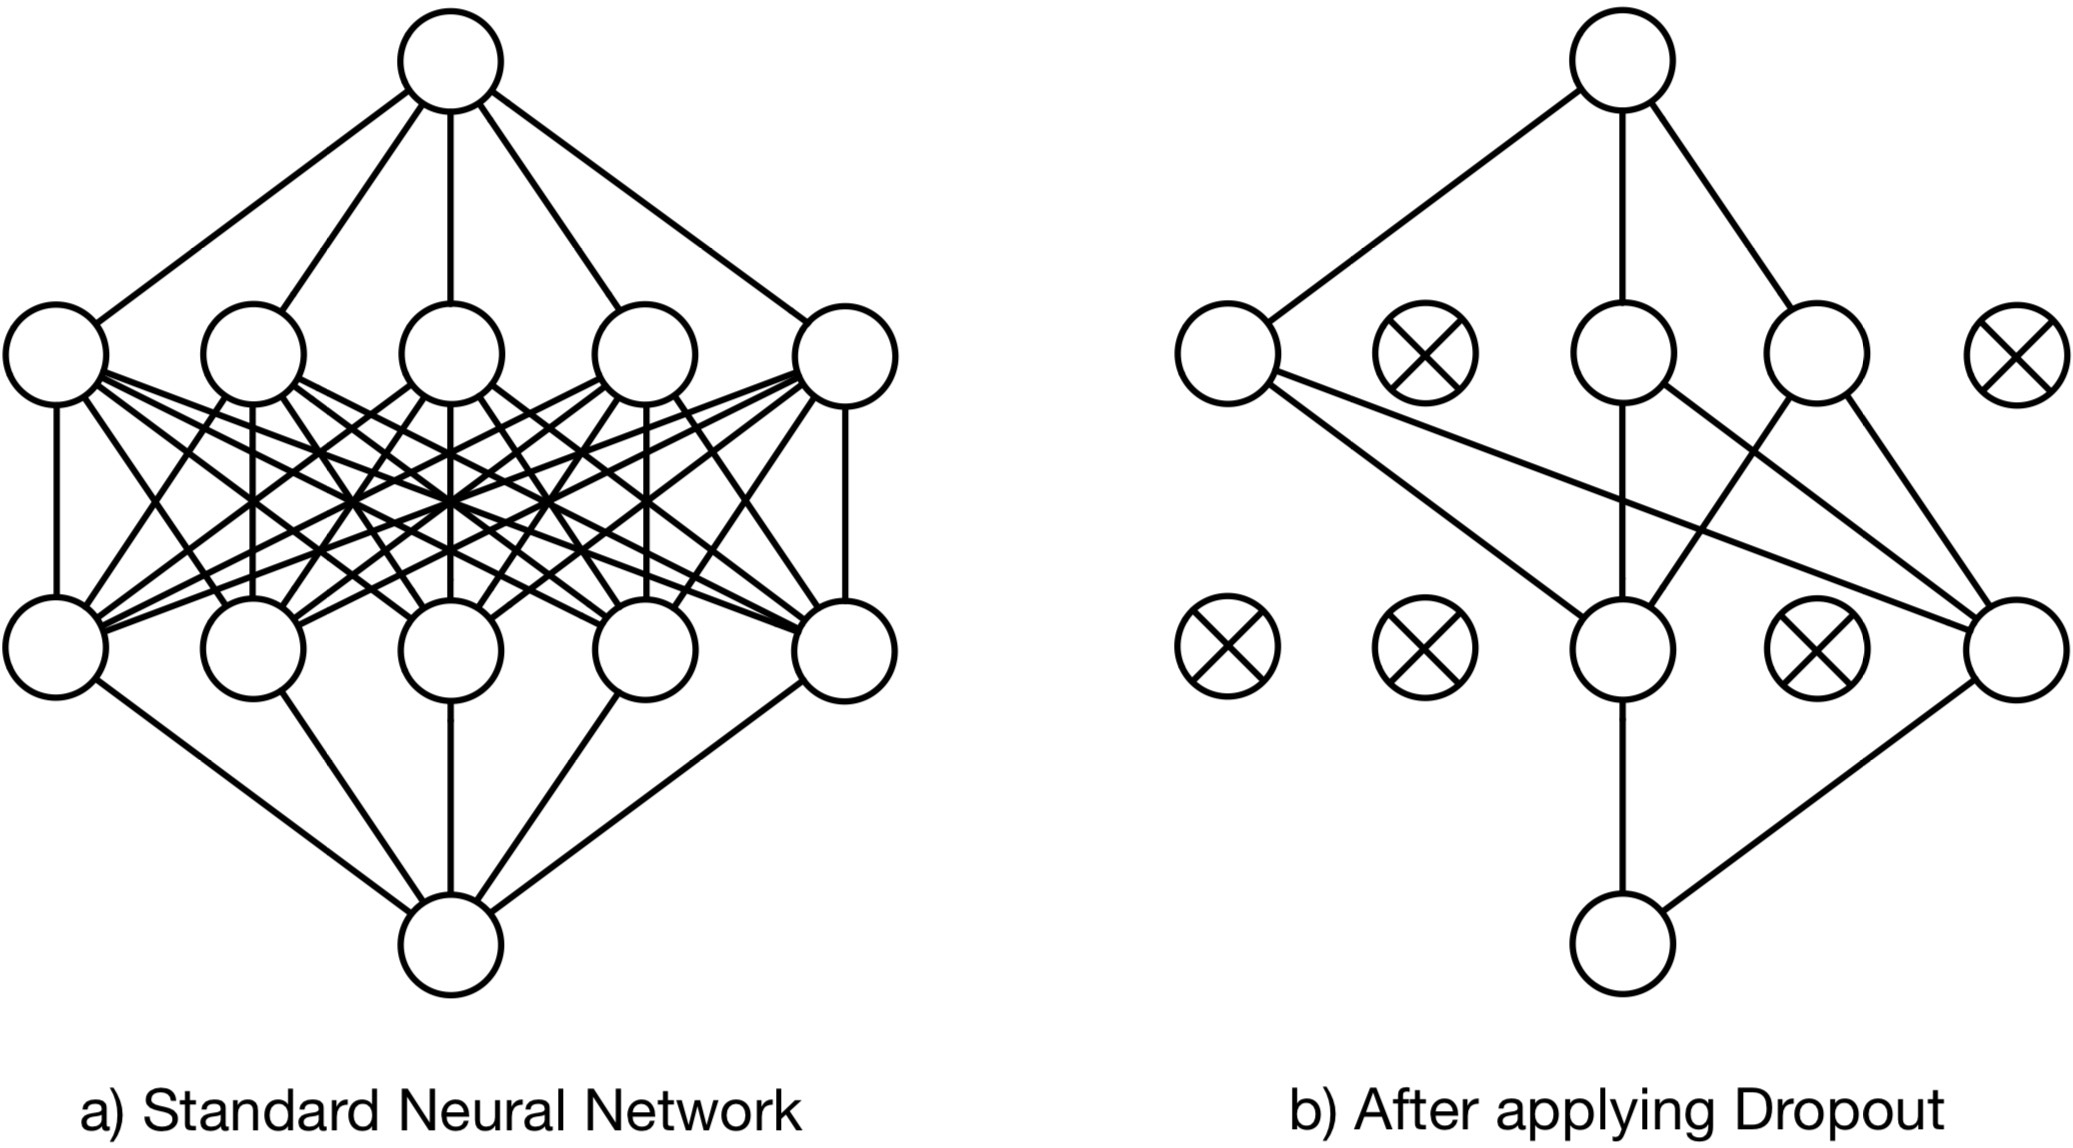
\includegraphics[width=0.65\linewidth]{figures/fig_dropout.png}
    \caption{Visualization of the dropout mechanism: (a) Standard neural network with two hidden layers; (b) Thinned network after applying dropout masks. Crossed neurons are temporarily deactivated during training.\\
    This figure was manually reillustrated with minor adjustments, the original version was published by \citet{srivastava2014dropout}}
    \label{fig:dropout-srivastava}
\end{figure}

At test time, averaging across all possible thinned subnetworks is infeasible due to the exponential
growth of possible configurations with increasing network size. Instead, dropout is disabled, resulting
in a single network. Each of the network's weights is scaled by $p$, which approximates the geometric
mean of predictions from all subnetworks without the heavy computation needed for explicit averaging.

\vspace{0.15cm}
Unlike Monte Carlo Dropout, standard dropout functions purely as a regularizer, which means it
improves generalization and reduces overfitting but doesn't provide uncertainty estimates
\citep{srivastava2014dropout}.


\subsection{Monte Carlo Dropout}
\label{methodology:mcd}
\citet{gal2016mcdropout} introduced Monte Carlo dropout (MC-Dropout) as an efficient method to estimate
uncertainty in neural networks. Unlike classic dropout, MC-Dropout keeps dropout active during testing.
It performs multiple stochastic forward passes through the network, each with different randomly
activated neurons, effectively sampling predictions $\{f^{\hat{\mathbf{W}}_t}(x^*)\}_{t=1}^T$ from $T$
thinned subnetworks. Each subnetwork's weights $\hat{\mathbf{W}}_t$ can be thought of as a sample from
the posterior $p(\mathbf{W} \mid \mathcal{D})$ and each prediction $f^{\hat{\mathbf{W}}_t}(x^*)$ as a
sample from the predictive distribution $p(y^* \mid x^*, \mathcal{D})$. The predictive distribution
quantifies the uncertainty about the models response for a new observation $x^*$ given the observed data.

The collection of these predictions forms a distribution where the mean approximates the expected
output and the variance quantifies epistemic uncertainty. Tightly clustered predictions indicate
high confidence, while dispersed predictions reveal model uncertainty.

\begin{figure}[htbp]
    \centering
    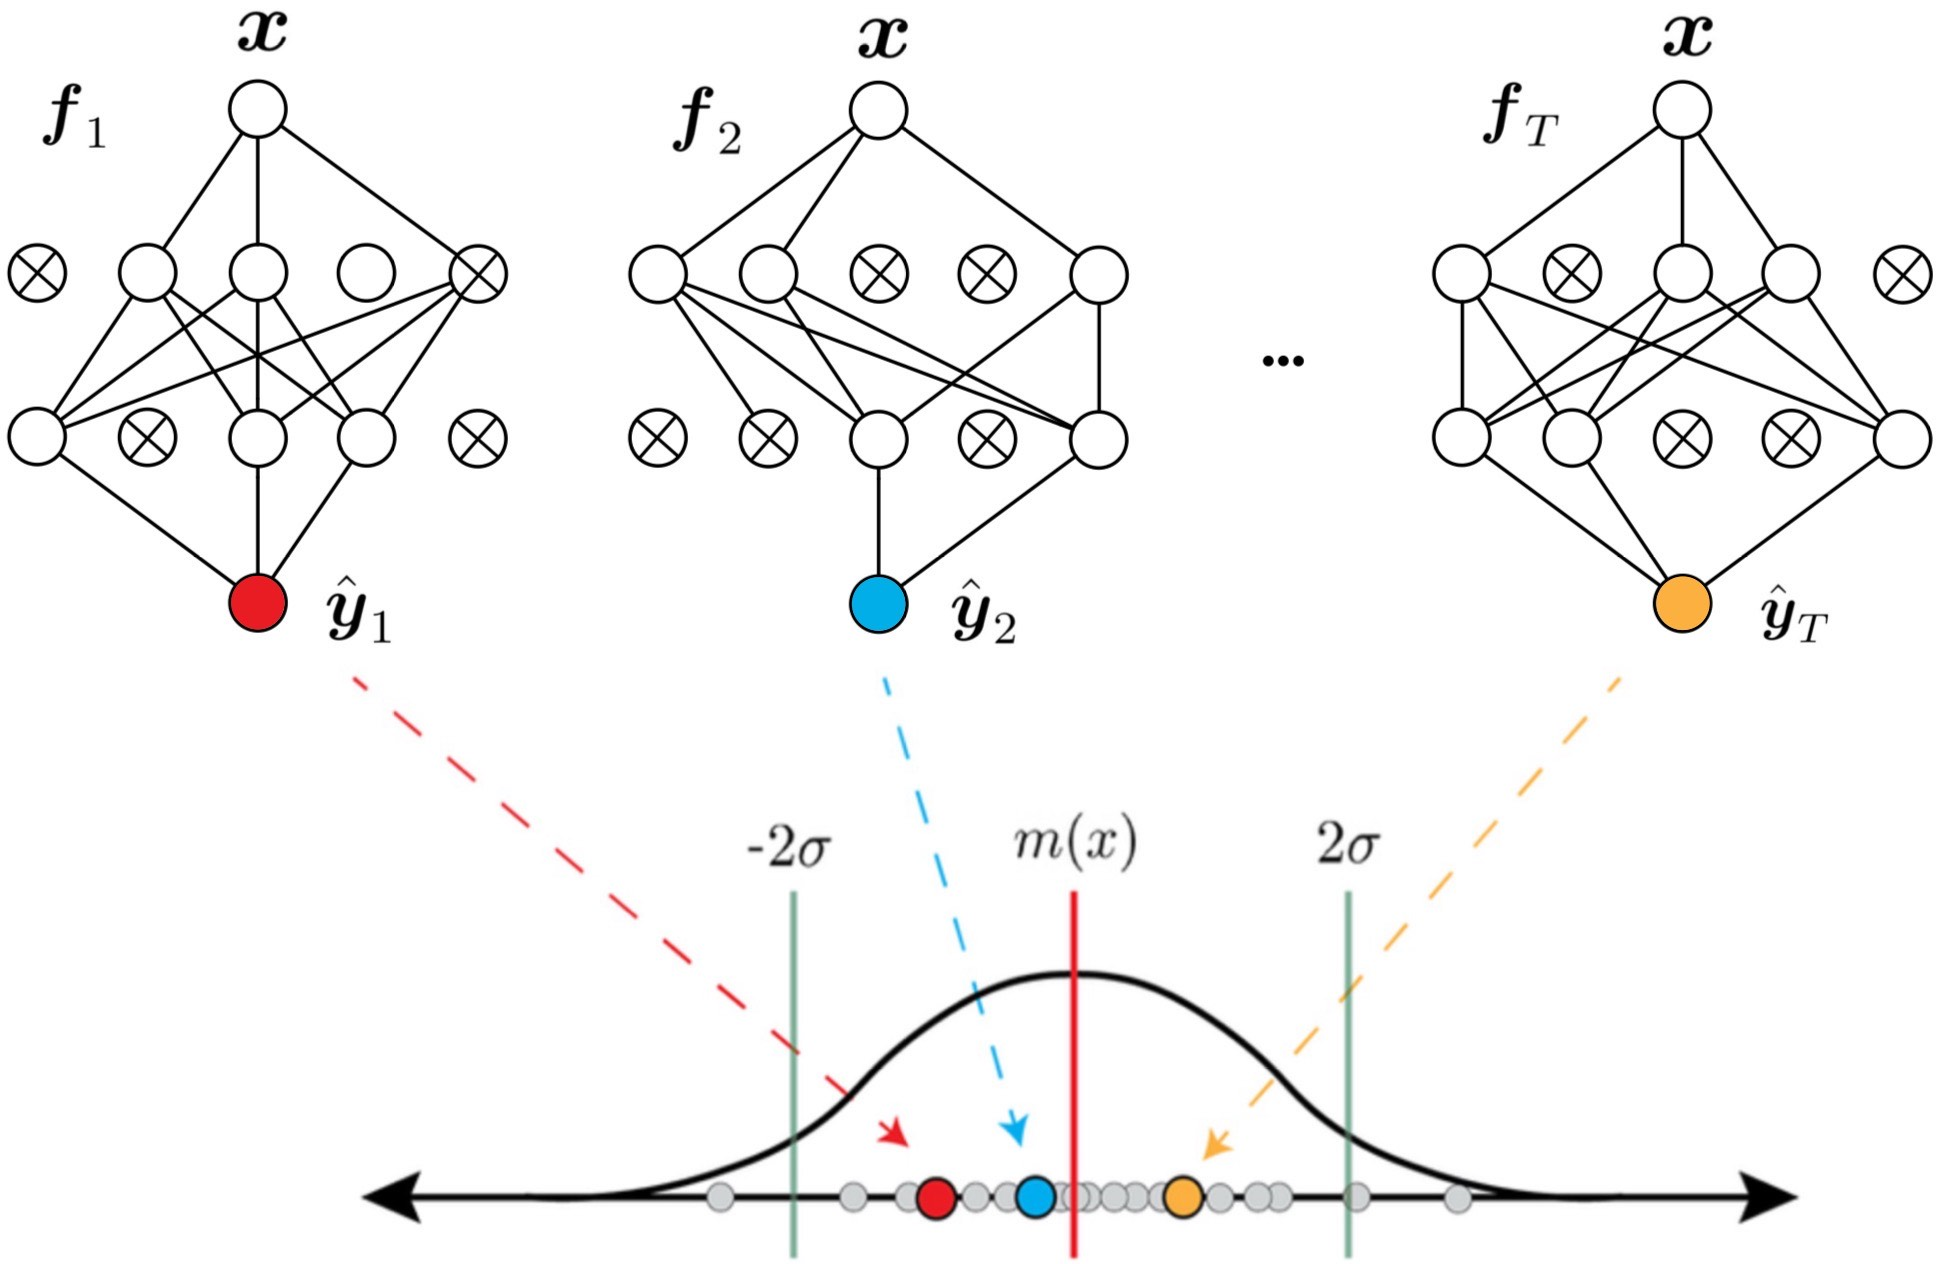
\includegraphics[width=0.65\linewidth]{figures/fig_mcd.png}
    \caption{MC-Dropouts predictive distribution. Colored and grey dots represent predictions from different thinned networks, crossed neurons are deactivated.\\This figure was manually reillustrated with minor adjustments, the original version was published by \citet{Katwyk2023}}
    \label{fig:mc-dropout2}
\end{figure}

MC-Dropout provides a Bayesian approximation without formal Bayesian neural networks.
By interpreting dropout as variational inference, it mimics posterior sampling through the predictive
distribution of subnetworks \citep{gal2016mcdropout}.

\vspace{0.15cm}
\textbf{Advantages:} MC-Dropout introduces minimal computational overhead since it requires only one
trained model and uses the same computational graph with dropout enabled during inference. It scales
efficiently, providing reasonable uncertainty estimates with significantly lower cost than full
ensembling. Implementation is straightforward in popular frameworks like PyTorch and TensorFlow.

\vspace{0.15cm}
\textbf{Limitations:} The method tends to underestimate uncertainty in data-sparse regions and may not
concentrate appropriately as the amount of data increases \citep{osband2016}.
The estimated uncertainty is sensitive to changes in hyperparameters (e.g. retention probability $p$)
\citep{verdoja2021behaviormcdropout}.
As a variational method, MC-Dropout primarily explores uncertainty around a single point (mode) in the
posterior space, potentially underestimating the true posteriors variance. This makes sense because the
diversity among subnetworks is low, since all of them are dropout versions of the main network.
In contrast, deep ensembles with independently trained models capture multiple modes, offering
greater predictive diversity and robustness to distribution shifts \citep{fort2020deepensembles}.

\vspace{0.15cm}
Despite its limitations, MC-Dropout remains a popular baseline for practical uncertainty quantification
due to its simplicity, low computational cost (especially compared to ensemble techniques, as the model
is trained only once), and compatibility with other uncertainty estimation methods. It is particularly
advantageous when training resources are limited or when the true posterior distribution is expected to be simple.


\subsection{Stochastic Weight Averaging Gaussian}
\label{methodology:swag}
Stochastic Weight Averaging with Gaussian posterior approximation (SWAG) builds on Stochastic Weight
Averaging (SWA), a technique introduced by \citet{izmailov2019swa}. The core idea behind SWA is,
that after training a neural network normally, one restarts stochastic gradient descent (SGD) from that
trained state using a constant or cyclical learning rate to explore the weight space. The weights $w_i$
obtained after each iteration $i$ of the SGD algorithm are periodically saved and once the algorithm
finishes after $T$ or more iterations, the SWA mean (or SWA solution) is computed:

\[
\mathbf{w}_{\mathrm{SWA}} = \frac{1}{T}\sum_{i=1}^T \mathbf{w}_i
\]

\citet{izmailov2019swa} argue, that the SWA mean converges toward the center of a wide, flat region in
the loss surface, which leads to a more robust model and better generalization compared to the solution
that conventional SGD produces.

\vspace{0.15cm}
SWAG \citep{maddox2019swag} extends SWA by constructing a Gaussian posterior approximation from these
weight snapshots. It estimates not just the mean $\mathbf{w}_{\mathrm{SWA}}$, but also a covariance
matrix capturing parameter uncertainty. The covariance comprises two complementary components:

\begin{enumerate}
    \item \textbf{Diagonal covariance ($\Sigma_{\mathrm{diag}}$):} Computes per-parameter variance\\
    $\Sigma_{\mathrm{diag}} = \mathrm{diag}\left(\frac{1}{T-1}\sum_{i=1}^T (\mathbf{w}_i - \mathbf{w}_{\mathrm{SWA}})^2\right)$.\\
    This captures independent uncertainty estimates for individual weights.
          
    \item \textbf{Low-rank covariance ($\Sigma_{\mathrm{low\text{-}rank}}$):} Constructed from deviation
    vectors\\
    $\Sigma_{\mathrm{low\text{-}rank}} = \frac{1}{2(T-1)}\mathbf{D}\mathbf{D}^\top$  
    where $\mathbf{D} = [\mathbf{w}_1 - \mathbf{w}_{\mathrm{SWA}}, \dots, \mathbf{w}_T - \mathbf{w}_{\mathrm{SWA}}]$.\\
    This low-rank approximation captures dominant correlations between parameters.
\end{enumerate}

The combined covariance $\Sigma = \Sigma_{\mathrm{diag}} + \Sigma_{\mathrm{low\text{-}rank}}$ addresses
limitations of purely diagonal approximations, which often underestimate uncertainty by ignoring
parameter correlations \citep{maddox2019swag}. The full posterior approximation is:

\[
q_{\mathrm{SWAG}}(\mathbf{w}) = \mathcal{N}\left(\mathbf{w}_\mathrm{SWA}, \Sigma_\mathrm{diag} + \Sigma_\mathrm{low\text{-}rank}\right)
\]

At test time, SWAG samples weights $\mathbf{w}^{(s)} \sim q_{\mathrm{SWAG}}$ and computes predictions
$f^{\mathbf{w}^{(s)}}(x^*)$ for each sample. The resulting empirical distribution estimates the
predictive distribution $p(y^* \mid x^*, \mathcal{D})$, which as stated in Section \ref{methodology:mcd}
quantifies the uncertainty about the models response for a new observation given the observed data, its
mean approximates the expected output and its variance the epistemic uncertainty.

\vspace{0.15cm}
\textbf{Advantages:} By analyzing the SGD weight trajectories, SWAG captures posterior structure around
flat minima in the loss surface. While more computationally intensive than MC-Dropout, since it requires
extended training for weight exploration and covariance calculation, it remains significantly cheaper
than full ensembles because only one model is trained. \citet{maddox2019swag} demonstrate its superior
uncertainty calibration and robustness to distribution shifts compared to MC-Dropout and other
baselines, particularly on vision benchmarks like CIFAR and ImageNet.

\vspace{0.15cm}
\textbf{Limitations:} Although SWAG approximates uncertainty better than simpler methods, it still,
similar to MC-Dropout, represents a single mode of the posterior and does not learn true multimodal
structures \citep{onal2024multiswag}. Memory requirements increase with snapshot frequency due to
covariance storage, though remain manageable versus full ensembles. The quality of the uncertainty
estimation depends on the learning rate set for the exploration phase \citep{maddox2019swag}.

\vspace{0.15cm}
SWAG thus provides an efficient midpoint between simple variational methods and computationally
intensive approaches, offering structured uncertainty estimation with minimal training overhead beyond
standard SGD.
\newpage
